Commands are sent to the ez\-L\-C\-D though the serial interface, Commands are text based and end with a carrage return {\bfseries cr}.\par
 So if you send {\bfseries cls} ending with a {\bfseries cr} the device will clear the screen and return a {\bfseries cr} when the command is complete,\par
 some widgets take a bit of time (in the millsecond range) to complete so after sending a command allways wait for a {\bfseries cr} to comeback before sending another command.\par
 

\par
 Minimal example will open the ez\-L\-C\-D port clear the screen and print 'Hello From Python' in red \par
  
\begin{DoxyImageNoCaption}
  \mbox{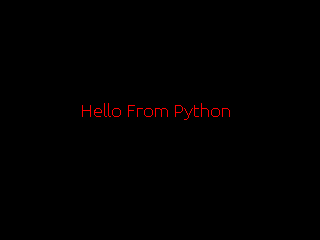
\includegraphics{minimal.png}}
\end{DoxyImageNoCaption}
 
\begin{DoxyCodeInclude}
1 \textcolor{comment}{# Minimal ezLCD Python demo}
2 \textcolor{comment}{#}
3 
4 \textcolor{keyword}{import} platform
5 \textcolor{keyword}{import} sys
6 
7 
8 sys.path.append(\textcolor{stringliteral}{"C:\(\backslash\)Users\(\backslash\)codeman\(\backslash\)Documents\(\backslash\)GitHub\(\backslash\)ezLCD3xxPython\(\backslash\)module"}) 
9 \textcolor{keyword}{from} ezLCD3xx \textcolor{keyword}{import} *
10 
11 \textcolor{comment}{#check what OS we are on}
12 \textcolor{comment}{#Windows}
13 \textcolor{keywordflow}{if} platform.system() == \textcolor{stringliteral}{'Windows'}:
14     LCD = ezLCD(\textcolor{stringliteral}{'com6'}) 
15 \textcolor{comment}{#Mac}
16 \textcolor{keywordflow}{elif} platform.system() == \textcolor{stringliteral}{'Dawrwin'}:
17     LCD = ezLCD(\textcolor{stringliteral}{'/dev/tty.usbsomething'})
18 \textcolor{comment}{# Bail out if comport error}
19 \textcolor{keywordflow}{if} LCD.openSerial()==\textcolor{keyword}{False}:
20     \textcolor{keywordflow}{print} \textcolor{stringliteral}{'Error Opening Port'}
21     \textcolor{keywordflow}{raise} SystemExit
22 
23 \textcolor{comment}{# Turn verbose off }
24 LCD.verbose(\textcolor{stringliteral}{'off'})
25 \textcolor{comment}{# Turn off button press info from ezLCD}
26 LCD.wquiet(ON)
27 \textcolor{comment}{# CLear screen}
28 LCD.cls()
29 \textcolor{comment}{# Set draw color to red}
30 LCD.color(RED)
31 \textcolor{comment}{# Print string at coordinates x=80 and y=100}
32 LCD.printString(\textcolor{stringliteral}{"Hello From Python"},80,100)
33 
\end{DoxyCodeInclude}
 Button example will display a button widget then poll for button presses and update screen \par
  
\begin{DoxyImageNoCaption}
  \mbox{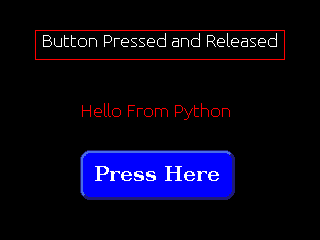
\includegraphics{button.png}}
\end{DoxyImageNoCaption}
 
\begin{DoxyCodeInclude}
1 \textcolor{comment}{# Button ezLCD Python demo}
2 \textcolor{comment}{#}
3 
4 \textcolor{keyword}{import} platform
5 \textcolor{keyword}{import} sys
6 sys.path.append(\textcolor{stringliteral}{'module'}) 
7 \textcolor{keyword}{from} ezLCD3xx \textcolor{keyword}{import} *
8 
9 \textcolor{comment}{#check what OS we are on}
10 \textcolor{comment}{#Windows}
11 \textcolor{keywordflow}{if} platform.system() == \textcolor{stringliteral}{'Windows'}:
12     LCD = ezLCD(\textcolor{stringliteral}{'com4'}) 
13 \textcolor{comment}{#Mac}
14 \textcolor{keywordflow}{elif} platform.system() == \textcolor{stringliteral}{'Dawrwin'}:
15     LCD = ezLCD(\textcolor{stringliteral}{'/dev/tty.usbsomething'})
16 \textcolor{comment}{#Linux}
17 \textcolor{keywordflow}{elif} platform.system() == \textcolor{stringliteral}{'Linux'}:
18     LCD = ezLCD(\textcolor{stringliteral}{'/dev/ttyACM0'})
19 
20 \textcolor{comment}{# Bail out if comport error}
21 \textcolor{keywordflow}{if} LCD.openSerial()==\textcolor{keyword}{False}:
22     \textcolor{keywordflow}{print} \textcolor{stringliteral}{'Error Opening Port'}
23     \textcolor{keywordflow}{raise} SystemExit
24 
25 \textcolor{comment}{# Turn verbose off }
26 LCD.verbose(\textcolor{stringliteral}{'off'})
27 \textcolor{comment}{# Turn off button press info from ezLCD}
28 LCD.wquiet(ON)
29 \textcolor{comment}{# CLear screen}
30 LCD.cls()
31 \textcolor{comment}{# Set draw color to red}
32 LCD.color(RED)
33 \textcolor{comment}{# Set widget font 0}
34 LCD.fontw(0,\textcolor{stringliteral}{'1'})
35 \textcolor{comment}{# Set wodget font 1}
36 LCD.fontw(1,\textcolor{stringliteral}{'0'})
37 \textcolor{comment}{# Set theme #1 }
38 LCD.theme(1, 155, 152, 3, 0, 3, 24, 4, 5, 0, 1)
39 \textcolor{comment}{# Print string at coordinates x=80 and y=100}
40 LCD.printString(\textcolor{stringliteral}{"Hello From Python"},80,100)
41 \textcolor{comment}{# Draw button widget with a ID of 1}
42 LCD.button( 1,  80, 150, 155, 50, 1, 0, 10, 6, 3,\textcolor{stringliteral}{'Press Here'})
43 \textcolor{comment}{# Draw a staticText box}
44 LCD.staticText(2, 35, 30, 250, 30, 8, 1, 1,\textcolor{stringliteral}{'Press Button'})
45 \textcolor{comment}{# Clear widget stack}
46 LCD.wstack(CLEAR)
47 
48 \textcolor{keywordflow}{while} \textcolor{keyword}{True}:
49     \textcolor{comment}{# check widget stack this will return widget updates (button press ect.) last in first out order}
50     (ID, Info, Data) = LCD.wstack(LIFO)
51 \textcolor{comment}{#   print ID, Info, Data}
52     \textcolor{comment}{# check if ID = 1 widget 1 and info = pressed }
53     \textcolor{keywordflow}{if} ID == 1 \textcolor{keywordflow}{and} Info == 4:
54         \textcolor{comment}{# clear the stack just to be safe}
55 \textcolor{comment}{#       LCD.wstack(CLEAR)}
56         \textcolor{comment}{# change draw color to yellow}
57         LCD.color(YELLOW)
58         \textcolor{comment}{# change change string 1 for text on static text ID 2}
59         LCD.string(1,\textcolor{stringliteral}{'Button Pressed'})
60         \textcolor{comment}{# redraw static text box ID 2 3=redraw      }
61         LCD.wstate(2, 3)
62     \textcolor{comment}{# check if ID = 1 widget 1 and info = pressed and released}
63     \textcolor{keywordflow}{if} ID == 1 \textcolor{keywordflow}{and} Info == 1:
64         \textcolor{comment}{# clear the stack just to be safe}
65 \textcolor{comment}{#       LCD.wstack(CLEAR)}
66         \textcolor{comment}{# change draw color to yellow}
67         LCD.color(YELLOW)
68         \textcolor{comment}{# change change string 1 for text on static text ID 2}
69         LCD.string(1,\textcolor{stringliteral}{'Button Pressed and Released'})
70         \textcolor{comment}{# redraw static text box ID 2 3=redraw}
71         LCD.wstate(2, 3)
72 
73         
\end{DoxyCodeInclude}
 Load example will display the cpu load as a graph \par
  
\begin{DoxyImageNoCaption}
  \mbox{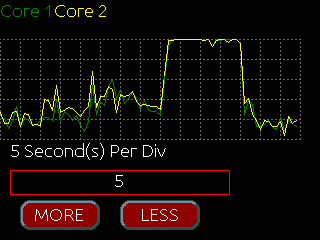
\includegraphics{load.png}}
\end{DoxyImageNoCaption}
 
\begin{DoxyCodeInclude}
1 \textcolor{comment}{#!/usr/bin/env python}
2 \textcolor{comment}{# Python Serial library for ezLCD3xx}
3 \textcolor{comment}{# http://www.ezlcd.com/}
4 \textcolor{comment}{#}
5 \textcolor{comment}{# You need the pySerial Library by Chris Liechti}
6 \textcolor{comment}{# http://pyserial.wiki.sourceforge.net/pySerial}
7 \textcolor{comment}{#}
8 
9 
10 \textcolor{comment}{# END SerLCD Class Definition --------------------------------------}
11 
12 \textcolor{comment}{# Start Test Program -----------------------------------------------}
13 \textcolor{keyword}{import} commands
14 \textcolor{keyword}{import} os
15 \textcolor{keyword}{import} re
16 \textcolor{keyword}{import} time \textcolor{keyword}{as} timer
17 \textcolor{keyword}{import} sys
18 \textcolor{keyword}{import} platform
19 \textcolor{keyword}{import} time
20 \textcolor{keyword}{import} psutil
21     
22 sys.path.append(\textcolor{stringliteral}{'module'}) 
23 \textcolor{keyword}{from} ezLCD3xx \textcolor{keyword}{import} *
24 
25 \textcolor{keyword}{def }drawGrid():
26     LCD.lineType(2)
27     LCD.xy(0,30)
28     LCD.color(BLACK)
29     LCD.box(300,110,1)
30     LCD.xy(0,0)
31     LCD.color(GREEN)
32     LCD.printString(\textcolor{stringliteral}{'Core 1'})
33     LCD.color(YELLOW)
34     LCD.printString(\textcolor{stringliteral}{'Core 2'})
35     LCD.color(155)
36     LCD.color(LIME)
37     LCD.font(\textcolor{stringliteral}{'1'})
38     LCD.font(\textcolor{stringliteral}{'0'})
39     LCD.color(151)
40     \textcolor{keywordflow}{for} y \textcolor{keywordflow}{in} range(6):
41         LCD.xy(0,(y*20)+39)
42         LCD.line(300,(y*20)+39)
43     \textcolor{keywordflow}{for} x \textcolor{keywordflow}{in} range(16):
44         LCD.xy(x*20,39)
45         LCD.line(x*20,139)
46     LCD.xy(300,39)
47     LCD.line(300,139)
48     LCD.lineType(0)
49     
50 \textcolor{keyword}{def }drawTime(res):
51     LCD.xy(10,140)
52     LCD.color(BLACK)
53     LCD.box(300,30, FILLED)
54     LCD.color(WHITE)
55     Time=str(res)+\textcolor{stringliteral}{' Second(s) Per Div'}
56     LCD.printString(Time)
57 
58     LCD.string(5, str(res))
59     LCD.wstate(7,REDRAW)
60 
61 
62 \textcolor{comment}{#check what OS we are on}
63 \textcolor{comment}{#Windows}
64 \textcolor{keywordflow}{if} platform.system() == \textcolor{stringliteral}{'Windows'}:
65     LCD = ezLCD(\textcolor{stringliteral}{'com6'}) 
66 \textcolor{comment}{#Mac}
67 \textcolor{keywordflow}{elif} platform.system() == \textcolor{stringliteral}{'Dawrwin'}:
68     LCD = ezLCD(\textcolor{stringliteral}{'/dev/tty.usbsomething'})
69 \textcolor{comment}{#Linux}
70 \textcolor{keywordflow}{elif} platform.system() == \textcolor{stringliteral}{'Linux'}:
71     LCD = ezLCD(\textcolor{stringliteral}{'/dev/ttyACM0'})
72 \textcolor{comment}{# Bail out if comport error}
73 \textcolor{keywordflow}{if} LCD.openSerial()==\textcolor{keyword}{False}:
74     \textcolor{keywordflow}{print} \textcolor{stringliteral}{'Error Opening Port'}
75     \textcolor{keywordflow}{raise} SystemExit
76 
77 LCD.ping()
78 LCD.verbose(\textcolor{stringliteral}{'OFF'})
79 LCD.wquiet(ON)
80 LCD.cls()
81 LCD.fontw(0,\textcolor{stringliteral}{'1'})
82 LCD.fontw(1,\textcolor{stringliteral}{'0'})
83 LCD.fontw(2,\textcolor{stringliteral}{'serif24'})
84 LCD.theme(1, 155, 152, 3, 0, 3, 24, 4, 5, 0, 1)
85 LCD.backlight(100, 5, 10)
86 LCD.cls()
87 LCD.font(\textcolor{stringliteral}{'0'})
88 LCD.fonto(0)
89 info = \textcolor{stringliteral}{' '}
90 LCD.string( 1, \textcolor{stringliteral}{'%'})
91 LCD.color(WHITE)
92 LCD.cfgio(8,\textcolor{stringliteral}{'analog'})
93 \textcolor{keywordflow}{print} LCD.xmax()
94 \textcolor{keywordflow}{print} LCD.ymax()
95 LCD.xy(100,100)
96 (x,y) = LCD.xy()
97 \textcolor{keywordflow}{print} int(x), int(y)
98 (r,g,b)=LCD.colorId(3)
99 \textcolor{keywordflow}{print} r,g,b
100 \textcolor{keywordflow}{print} LCD.string(65)
101 \textcolor{keywordflow}{print} LCD.string(66)
102 \textcolor{keywordflow}{print} LCD.color()
103 \textcolor{keywordflow}{print} LCD.io(8)
104 
105 
106 LCD.button( 5, 20, 200, 80, 30 , 1, 0, 10, 1, 2, \textcolor{stringliteral}{'MORE'})
107 LCD.button( 6, 120, 200, 80, 30 , 1, 0, 10, 1, 3, \textcolor{stringliteral}{'LESS'})
108 LCD.staticText(7, 10, 170, 220, 25, 8, 1, 5, \textcolor{stringliteral}{'test'})
109 drawGrid()
110 x=0
111 y1=239
112 y2=239
113 lx=0
114 ly1=239
115 ly2=239
116 res=5
117 drawTime(res)   
118 LCD.wstack(CLEAR)     
119 \textcolor{keywordflow}{while} \textcolor{keyword}{True}:
120 
121     oldinfo = info
122     cores=psutil.cpu\_percent(interval=1, percpu=\textcolor{keyword}{True})
123     y1 = 139 - cores[0]
124     y2 = 139 - cores[1]
125     \textcolor{keywordflow}{if} x!=0:
126         LCD.color(GREEN)
127         LCD.xy(lx,ly1)
128         LCD.line(x, y1)
129         LCD.color(YELLOW)
130         LCD.xy(lx,ly2)
131         LCD.line(x, y2)
132     ly1 = y1
133     ly2 = y2
134     lx = x   
135     x += 20/res
136     
137     \textcolor{keywordflow}{if} x >= 300:
138         x=0
139         y1=239
140         y2=239
141         lx =0
142         ly1 =239
143         ly2 =239
144         drawGrid()
145     (ID, info, data) = LCD.wstack(LIFO)
146     LCD.wstack(CLEAR)
147     \textcolor{keywordflow}{if} ID == 5 \textcolor{keywordflow}{and} info==1:
148         res +=1
149         drawTime(res)  
150     \textcolor{keywordflow}{if} ID == 6 \textcolor{keywordflow}{and} info==1:
151         \textcolor{keywordflow}{if} res > 1:
152             res -=1
153             drawTime(res)
154 LCD.closeSerial()
155 \textcolor{comment}{# End Test Program --------------------------------------}
\end{DoxyCodeInclude}
 